% Options for packages loaded elsewhere
\PassOptionsToPackage{unicode}{hyperref}
\PassOptionsToPackage{hyphens}{url}
%
\documentclass[
]{article}
\usepackage{amsmath,amssymb}
\usepackage{lmodern}
\usepackage{ifxetex,ifluatex}
\ifnum 0\ifxetex 1\fi\ifluatex 1\fi=0 % if pdftex
  \usepackage[T1]{fontenc}
  \usepackage[utf8]{inputenc}
  \usepackage{textcomp} % provide euro and other symbols
\else % if luatex or xetex
  \usepackage{unicode-math}
  \defaultfontfeatures{Scale=MatchLowercase}
  \defaultfontfeatures[\rmfamily]{Ligatures=TeX,Scale=1}
\fi
% Use upquote if available, for straight quotes in verbatim environments
\IfFileExists{upquote.sty}{\usepackage{upquote}}{}
\IfFileExists{microtype.sty}{% use microtype if available
  \usepackage[]{microtype}
  \UseMicrotypeSet[protrusion]{basicmath} % disable protrusion for tt fonts
}{}
\makeatletter
\@ifundefined{KOMAClassName}{% if non-KOMA class
  \IfFileExists{parskip.sty}{%
    \usepackage{parskip}
  }{% else
    \setlength{\parindent}{0pt}
    \setlength{\parskip}{6pt plus 2pt minus 1pt}}
}{% if KOMA class
  \KOMAoptions{parskip=half}}
\makeatother
\usepackage{xcolor}
\IfFileExists{xurl.sty}{\usepackage{xurl}}{} % add URL line breaks if available
\IfFileExists{bookmark.sty}{\usepackage{bookmark}}{\usepackage{hyperref}}
\hypersetup{
  pdftitle={MATH 4322 Homework 1},
  pdfauthor={Phu Nguyen},
  hidelinks,
  pdfcreator={LaTeX via pandoc}}
\urlstyle{same} % disable monospaced font for URLs
\usepackage[margin=1in]{geometry}
\usepackage{color}
\usepackage{fancyvrb}
\newcommand{\VerbBar}{|}
\newcommand{\VERB}{\Verb[commandchars=\\\{\}]}
\DefineVerbatimEnvironment{Highlighting}{Verbatim}{commandchars=\\\{\}}
% Add ',fontsize=\small' for more characters per line
\usepackage{framed}
\definecolor{shadecolor}{RGB}{248,248,248}
\newenvironment{Shaded}{\begin{snugshade}}{\end{snugshade}}
\newcommand{\AlertTok}[1]{\textcolor[rgb]{0.94,0.16,0.16}{#1}}
\newcommand{\AnnotationTok}[1]{\textcolor[rgb]{0.56,0.35,0.01}{\textbf{\textit{#1}}}}
\newcommand{\AttributeTok}[1]{\textcolor[rgb]{0.77,0.63,0.00}{#1}}
\newcommand{\BaseNTok}[1]{\textcolor[rgb]{0.00,0.00,0.81}{#1}}
\newcommand{\BuiltInTok}[1]{#1}
\newcommand{\CharTok}[1]{\textcolor[rgb]{0.31,0.60,0.02}{#1}}
\newcommand{\CommentTok}[1]{\textcolor[rgb]{0.56,0.35,0.01}{\textit{#1}}}
\newcommand{\CommentVarTok}[1]{\textcolor[rgb]{0.56,0.35,0.01}{\textbf{\textit{#1}}}}
\newcommand{\ConstantTok}[1]{\textcolor[rgb]{0.00,0.00,0.00}{#1}}
\newcommand{\ControlFlowTok}[1]{\textcolor[rgb]{0.13,0.29,0.53}{\textbf{#1}}}
\newcommand{\DataTypeTok}[1]{\textcolor[rgb]{0.13,0.29,0.53}{#1}}
\newcommand{\DecValTok}[1]{\textcolor[rgb]{0.00,0.00,0.81}{#1}}
\newcommand{\DocumentationTok}[1]{\textcolor[rgb]{0.56,0.35,0.01}{\textbf{\textit{#1}}}}
\newcommand{\ErrorTok}[1]{\textcolor[rgb]{0.64,0.00,0.00}{\textbf{#1}}}
\newcommand{\ExtensionTok}[1]{#1}
\newcommand{\FloatTok}[1]{\textcolor[rgb]{0.00,0.00,0.81}{#1}}
\newcommand{\FunctionTok}[1]{\textcolor[rgb]{0.00,0.00,0.00}{#1}}
\newcommand{\ImportTok}[1]{#1}
\newcommand{\InformationTok}[1]{\textcolor[rgb]{0.56,0.35,0.01}{\textbf{\textit{#1}}}}
\newcommand{\KeywordTok}[1]{\textcolor[rgb]{0.13,0.29,0.53}{\textbf{#1}}}
\newcommand{\NormalTok}[1]{#1}
\newcommand{\OperatorTok}[1]{\textcolor[rgb]{0.81,0.36,0.00}{\textbf{#1}}}
\newcommand{\OtherTok}[1]{\textcolor[rgb]{0.56,0.35,0.01}{#1}}
\newcommand{\PreprocessorTok}[1]{\textcolor[rgb]{0.56,0.35,0.01}{\textit{#1}}}
\newcommand{\RegionMarkerTok}[1]{#1}
\newcommand{\SpecialCharTok}[1]{\textcolor[rgb]{0.00,0.00,0.00}{#1}}
\newcommand{\SpecialStringTok}[1]{\textcolor[rgb]{0.31,0.60,0.02}{#1}}
\newcommand{\StringTok}[1]{\textcolor[rgb]{0.31,0.60,0.02}{#1}}
\newcommand{\VariableTok}[1]{\textcolor[rgb]{0.00,0.00,0.00}{#1}}
\newcommand{\VerbatimStringTok}[1]{\textcolor[rgb]{0.31,0.60,0.02}{#1}}
\newcommand{\WarningTok}[1]{\textcolor[rgb]{0.56,0.35,0.01}{\textbf{\textit{#1}}}}
\usepackage{graphicx}
\makeatletter
\def\maxwidth{\ifdim\Gin@nat@width>\linewidth\linewidth\else\Gin@nat@width\fi}
\def\maxheight{\ifdim\Gin@nat@height>\textheight\textheight\else\Gin@nat@height\fi}
\makeatother
% Scale images if necessary, so that they will not overflow the page
% margins by default, and it is still possible to overwrite the defaults
% using explicit options in \includegraphics[width, height, ...]{}
\setkeys{Gin}{width=\maxwidth,height=\maxheight,keepaspectratio}
% Set default figure placement to htbp
\makeatletter
\def\fps@figure{htbp}
\makeatother
\setlength{\emergencystretch}{3em} % prevent overfull lines
\providecommand{\tightlist}{%
  \setlength{\itemsep}{0pt}\setlength{\parskip}{0pt}}
\setcounter{secnumdepth}{-\maxdimen} % remove section numbering
\ifluatex
  \usepackage{selnolig}  % disable illegal ligatures
\fi

\title{MATH 4322 Homework 1}
\author{Phu Nguyen}
\date{9/4/2021}

\begin{document}
\maketitle

\hypertarget{problem-1}{%
\subsection{Problem 1}\label{problem-1}}

Explain whether each scenario is a classification or regression
problem,and indicate whether we are most interested in inference or
prediction. Finally, provide \(n\) number of observations and \(p\)
number of variables.

\begin{enumerate}
\def\labelenumi{(\alph{enumi})}
\tightlist
\item
  We collect a set of data on the top 500 firms in the US. For each firm
  we record profit, number of employees, industry and the CEO salary. We
  are interested in understanding which factors affect CEO salary.
\end{enumerate}

\begin{itemize}
\tightlist
\item
  \textbf{Answer}: This is a regression problem because the response
  `output' is the CEO salary and it's a quantitative value. We are most
  interested in inference because the factors that affect CEO salary is
  number of employees, and industry. We are interested in the way the
  \(Y\) which is the CEO salary is affected as \(X\) changes.
  \(n = 500\) and \(p = 3\).
\end{itemize}

\begin{enumerate}
\def\labelenumi{(\alph{enumi})}
\setcounter{enumi}{1}
\tightlist
\item
  We are considering launching a new product and wish to know whether it
  will be a success or a failure. We collect data on 20 similar products
  that were previously launched. For each product we have recorded
  whether it was a success or failure, price charged for the product,
  marketing budget, competition price, and ten other variables.
\end{enumerate}

\begin{itemize}
\tightlist
\item
  \textbf{Answer}: This is a classification problem because the response
  is a qualitative value, which means no arithmetic operation can be
  done. Here we are interested in predicting the
  \(\hat{Y} = \hat{f}(X)\), where \(\hat{f}\) is often treated as a
  \(black box\) The response is success or failures \(n = 20\) and
  \(p = 13\).
\end{itemize}

\begin{enumerate}
\def\labelenumi{(\alph{enumi})}
\setcounter{enumi}{2}
\tightlist
\item
  We are interested in predicting the percent of change in the USD/Euro
  exchange rate in relation to the weekly changes in the world stock
  markets. We collect weekly data for all of 2012. For each week we
  record the percent of change in the USD/Euro, the percent of change in
  the US market, the percent of change in the British market, and the
  percent of change in the German market.
\end{enumerate}

\begin{itemize}
\tightlist
\item
  \textbf{Answer}: This is a regression problem because the response is
  the USD/Euro exchange rate. Variables are US market, British market,
  and German market, therefore \(p = 3\). The number of observation is
  weekly, so in year 2012 there is 365/7 = 52, therefore \(n = 52\).
\end{itemize}

\hypertarget{problem-2}{%
\subsection{Problem 2}\label{problem-2}}

You will now think of some real-life applications for statistical
learning. Think of ones other than what your friends have.

\begin{enumerate}
\def\labelenumi{(\alph{enumi})}
\tightlist
\item
  Describe three real-life applications in which \(classification\)
  might be useful. Describe the response, as well as the predictors. Is
  the goal of each application inference or prediction? Explain your
  answer.
\end{enumerate}

\begin{itemize}
\item
  \begin{enumerate}
  \def\labelenumi{(\arabic{enumi})}
  \tightlist
  \item
    Check the weather if today is rainy or not rainy day. This can be
    predict by inputs of different type data, and we can get the data
    from the weather database. This application is inference because
    \(\hat{f}\) is known.
  \end{enumerate}
\item
  \begin{enumerate}
  \def\labelenumi{(\arabic{enumi})}
  \setcounter{enumi}{1}
  \tightlist
  \item
    Analyze images if a person is young or old. We can build a machine
    learning and feed it information of young and people. So that the
    machine can classify the difference between the two. This
    application is inference because \(\hat{f}\) is known.
  \end{enumerate}
\item
  \begin{enumerate}
  \def\labelenumi{(\arabic{enumi})}
  \setcounter{enumi}{2}
  \tightlist
  \item
    Speech recognition, we can have a machine learning that learn how
    human talk and learn the different frequency that each person
    produce. It can analyze if you're actually who you are when
    speaking. This is a prediction application because \(\hat{f}\) is a
    \(black box\) here.
  \end{enumerate}
\end{itemize}

\begin{enumerate}
\def\labelenumi{(\alph{enumi})}
\setcounter{enumi}{1}
\tightlist
\item
  Describe three real-life applications in which \(regression\) might be
  useful. Describe the response, as well as the predictors. Is the goal
  of each application inference or prediction? Explain your answer.
\end{enumerate}

\begin{itemize}
\item
  \begin{enumerate}
  \def\labelenumi{(\arabic{enumi})}
  \tightlist
  \item
    House price, we can predict the house price by when it was build,
    the area around it, number of floors, materials, etc\ldots{} This is
    a inference because \(\hat{f}\) is known.
  \end{enumerate}
\item
  \begin{enumerate}
  \def\labelenumi{(\arabic{enumi})}
  \setcounter{enumi}{1}
  \tightlist
  \item
    Revenue, we can predict the revenue of a company by the number of
    sales. This is a inference because \(\hat{f}\) is known.
  \end{enumerate}
\item
  \begin{enumerate}
  \def\labelenumi{(\arabic{enumi})}
  \setcounter{enumi}{2}
  \tightlist
  \item
    Weight, we can predict a person's weight by their sex, heights and
    age. This is a prediction because \(\hat{f}\) is not known here.
  \end{enumerate}
\end{itemize}

\begin{enumerate}
\def\labelenumi{(\alph{enumi})}
\setcounter{enumi}{2}
\tightlist
\item
  Describe three real-life applications in which \(cluster\) analysis
  might be useful.\\
\end{enumerate}

\begin{itemize}
\item
  \begin{enumerate}
  \def\labelenumi{(\arabic{enumi})}
  \tightlist
  \item
    Volcano Studies, we studies different sites of volcano to see when
    it would erupted and determined the time and period to evacuated
    people.
  \end{enumerate}
\item
  \begin{enumerate}
  \def\labelenumi{(\arabic{enumi})}
  \setcounter{enumi}{1}
  \tightlist
  \item
    Earthquakes Studies, we studies the geographic of a land and gather
    data to determine the danger zone and evacuated people.
  \end{enumerate}
\item
  \begin{enumerate}
  \def\labelenumi{(\arabic{enumi})}
  \setcounter{enumi}{2}
  \tightlist
  \item
    City's houses, studies the values based on the geographic and
    locations.
  \end{enumerate}
\end{itemize}

\hypertarget{problem-3}{%
\subsection{Problem 3}\label{problem-3}}

What are the advantages and disadvantages of a very flexible (versus a
less flexible) approach for regression or classification? Under what
circumstances might a more flexible approach be preferred to a less
flexible approach? When might a less flexible approach be preferred?\\
* \textbf{Answer}: If we are mainly interested in inference, then the
less flexible are much more interpretable. For example, when inference
is the goal, the linear model may be good choice since it's easier to
understand the relationship between \(Y\) and \(X_1, X_2,...,X_p\). On
the other hand, the flexible approach, such as the splines and the
boosting methods can lead to such complicated estimates of \(f\) that it
is difficult to understand how any individual predictor is associated
with the response.

\hypertarget{problem-4}{%
\subsection{Problem 4}\label{problem-4}}

This exercise involves the \(mtcars\) data set looked at in class.

\begin{enumerate}
\def\labelenumi{(\alph{enumi})}
\tightlist
\item
  Which of the predictors are quantitative, and which are qualitative?
\end{enumerate}

\begin{Shaded}
\begin{Highlighting}[]
\FunctionTok{names}\NormalTok{(mtcars)}
\end{Highlighting}
\end{Shaded}

\begin{verbatim}
##  [1] "mpg"  "cyl"  "disp" "hp"   "drat" "wt"   "qsec" "vs"   "am"   "gear"
## [11] "carb"
\end{verbatim}

\begin{itemize}
\tightlist
\item
  \textbf{Quantitative}: mpg, disp, hp, drat, wt, qsec, gear, carb.
\item
  \textbf{Qualitative}: cyl, vs, am.\\
\end{itemize}

\begin{enumerate}
\def\labelenumi{(\alph{enumi})}
\setcounter{enumi}{1}
\tightlist
\item
  What is the \(range\) of each quantitative predictor? You can answer
  this using the \texttt{range()} function.
\end{enumerate}

\begin{Shaded}
\begin{Highlighting}[]
\FunctionTok{range}\NormalTok{(mtcars)}
\end{Highlighting}
\end{Shaded}

\begin{verbatim}
## [1]   0 472
\end{verbatim}

\begin{enumerate}
\def\labelenumi{(\alph{enumi})}
\setcounter{enumi}{2}
\tightlist
\item
  What is the mean and standard deviation of each quantitative
  predictor?\\
  \textbf{Means}
\end{enumerate}

\begin{verbatim}
## [1] 20.09062
\end{verbatim}

\begin{verbatim}
## [1] 230.7219
\end{verbatim}

\begin{verbatim}
## [1] 146.6875
\end{verbatim}

\begin{verbatim}
## [1] 3.596563
\end{verbatim}

\begin{verbatim}
## [1] 3.21725
\end{verbatim}

\begin{verbatim}
## [1] 17.84875
\end{verbatim}

\begin{verbatim}
## [1] 3.6875
\end{verbatim}

\begin{verbatim}
## [1] 2.8125
\end{verbatim}

\textbf{Standard Deviation}

\begin{verbatim}
## [1] 6.026948
\end{verbatim}

\begin{verbatim}
## [1] 123.9387
\end{verbatim}

\begin{verbatim}
## [1] 68.56287
\end{verbatim}

\begin{verbatim}
## [1] 0.5346787
\end{verbatim}

\begin{verbatim}
## [1] 0.9784574
\end{verbatim}

\begin{verbatim}
## [1] 1.786943
\end{verbatim}

\begin{verbatim}
## [1] 0.7378041
\end{verbatim}

\begin{verbatim}
## [1] 1.6152
\end{verbatim}

\begin{enumerate}
\def\labelenumi{(\alph{enumi})}
\setcounter{enumi}{3}
\tightlist
\item
  Now remove the 10th through 32nd observations. What is the range,
  mean, and standard deviation of each predictor in the subset of the
  data that remains?
\end{enumerate}

\begin{Shaded}
\begin{Highlighting}[]
\NormalTok{mtcars.rm }\OtherTok{=}\NormalTok{ mtcars[}\SpecialCharTok{{-}}\FunctionTok{c}\NormalTok{(}\DecValTok{10}\SpecialCharTok{:}\DecValTok{32}\NormalTok{),]}
\end{Highlighting}
\end{Shaded}

\begin{Shaded}
\begin{Highlighting}[]
\FunctionTok{range}\NormalTok{(mtcars.rm)}
\end{Highlighting}
\end{Shaded}

\begin{verbatim}
## [1]   0 360
\end{verbatim}

\textbf{Means}

\begin{verbatim}
## [1] 20.09062
\end{verbatim}

\begin{verbatim}
## [1] 230.7219
\end{verbatim}

\begin{verbatim}
## [1] 146.6875
\end{verbatim}

\begin{verbatim}
## [1] 3.596563
\end{verbatim}

\begin{verbatim}
## [1] 3.21725
\end{verbatim}

\begin{verbatim}
## [1] 17.84875
\end{verbatim}

\begin{verbatim}
## [1] 3.6875
\end{verbatim}

\begin{verbatim}
## [1] 2.8125
\end{verbatim}

\textbf{Standard Deviation}

\begin{verbatim}
## [1] 6.026948
\end{verbatim}

\begin{verbatim}
## [1] 123.9387
\end{verbatim}

\begin{verbatim}
## [1] 68.56287
\end{verbatim}

\begin{verbatim}
## [1] 0.5346787
\end{verbatim}

\begin{verbatim}
## [1] 0.9784574
\end{verbatim}

\begin{verbatim}
## [1] 1.786943
\end{verbatim}

\begin{verbatim}
## [1] 0.7378041
\end{verbatim}

\begin{verbatim}
## [1] 1.6152
\end{verbatim}

\begin{enumerate}
\def\labelenumi{(\alph{enumi})}
\setcounter{enumi}{4}
\tightlist
\item
  Using the full data set, investigate the predictors graphically,using
  scatterplots or other tools of your choice. Create some plots
  highlighting the relationships among the predictors. Comment on your
  findings.
\end{enumerate}

\begin{Shaded}
\begin{Highlighting}[]
\FunctionTok{plot}\NormalTok{(mtcars}\SpecialCharTok{$}\NormalTok{wt, mtcars}\SpecialCharTok{$}\NormalTok{mpg)}
\end{Highlighting}
\end{Shaded}

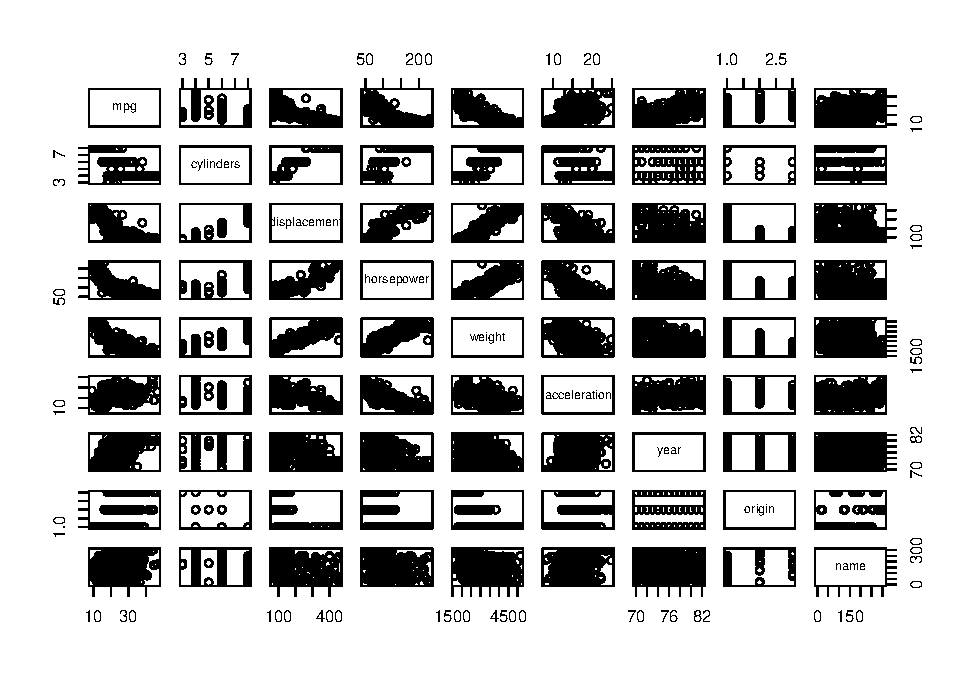
\includegraphics{hw1_fl21_files/figure-latex/unnamed-chunk-9-1.pdf} *
The relationship between \emph{wt} and \emph{mpg} is neative linear
relationsip

\begin{enumerate}
\def\labelenumi{(\alph{enumi})}
\setcounter{enumi}{5}
\tightlist
\item
  Suppose that we wish to predict gas mileage (mpg) on the basis of the
  other variables. Do your plots suggest that any of the other variables
  might be useful in predicting mpg? Justify your answer.
\end{enumerate}

\begin{Shaded}
\begin{Highlighting}[]
\NormalTok{mpglm.lm }\OtherTok{=} \FunctionTok{lm}\NormalTok{(mtcars}\SpecialCharTok{$}\NormalTok{mpg }\SpecialCharTok{\textasciitilde{}}\NormalTok{ mtcars}\SpecialCharTok{$}\NormalTok{disp }\SpecialCharTok{+}\NormalTok{ mtcars}\SpecialCharTok{$}\NormalTok{hp }\SpecialCharTok{+}\NormalTok{ mtcars}\SpecialCharTok{$}\NormalTok{drat }\SpecialCharTok{+}\NormalTok{ mtcars}\SpecialCharTok{$}\NormalTok{wt)}
\FunctionTok{summary}\NormalTok{(mpglm.lm)}
\end{Highlighting}
\end{Shaded}

\begin{verbatim}
## 
## Call:
## lm(formula = mtcars$mpg ~ mtcars$disp + mtcars$hp + mtcars$drat + 
##     mtcars$wt)
## 
## Residuals:
##     Min      1Q  Median      3Q     Max 
## -3.5077 -1.9052 -0.5057  0.9821  5.6883 
## 
## Coefficients:
##              Estimate Std. Error t value Pr(>|t|)    
## (Intercept) 29.148738   6.293588   4.631  8.2e-05 ***
## mtcars$disp  0.003815   0.010805   0.353  0.72675    
## mtcars$hp   -0.034784   0.011597  -2.999  0.00576 ** 
## mtcars$drat  1.768049   1.319779   1.340  0.19153    
## mtcars$wt   -3.479668   1.078371  -3.227  0.00327 ** 
## ---
## Signif. codes:  0 '***' 0.001 '**' 0.01 '*' 0.05 '.' 0.1 ' ' 1
## 
## Residual standard error: 2.602 on 27 degrees of freedom
## Multiple R-squared:  0.8376, Adjusted R-squared:  0.8136 
## F-statistic: 34.82 on 4 and 27 DF,  p-value: 2.704e-10
\end{verbatim}

\begin{itemize}
\tightlist
\item
  This model shows that beside from weight \emph{wt}, Gross horsepower
  \emph{hp} can be useful at predicting the \emph{mpg}
\end{itemize}

\hypertarget{problem-5}{%
\subsection{Problem 5}\label{problem-5}}

This exercise involves the Boston housing data set.

\begin{enumerate}
\def\labelenumi{(\alph{enumi})}
\tightlist
\item
  To begin, load in the Boston data set. The Boston data set is part of
  the \(MASS\) library in R.
\end{enumerate}

\begin{Shaded}
\begin{Highlighting}[]
\FunctionTok{library}\NormalTok{(MASS)}
\end{Highlighting}
\end{Shaded}

Now the data set is contained in the object Boston.

\begin{Shaded}
\begin{Highlighting}[]
\NormalTok{Boston}
\end{Highlighting}
\end{Shaded}

Read about the data set:

\begin{Shaded}
\begin{Highlighting}[]
\CommentTok{\#?Boston}
\end{Highlighting}
\end{Shaded}

How many rows are in this data set? How many columns? What do the rows
and columns represent?

\begin{Shaded}
\begin{Highlighting}[]
\FunctionTok{dim}\NormalTok{(Boston)}
\end{Highlighting}
\end{Shaded}

\begin{verbatim}
## [1] 506  14
\end{verbatim}

\begin{enumerate}
\def\labelenumi{(\alph{enumi})}
\setcounter{enumi}{1}
\tightlist
\item
  Make some pairwise scatterplots of the predictors (columns) in this
  data set. Describe your findings.
\end{enumerate}

\begin{Shaded}
\begin{Highlighting}[]
\FunctionTok{pairs}\NormalTok{(Boston[,}\FunctionTok{c}\NormalTok{(}\DecValTok{1}\SpecialCharTok{:}\DecValTok{3}\NormalTok{)])}
\end{Highlighting}
\end{Shaded}

\includegraphics{hw1_fl21_files/figure-latex/unnamed-chunk-15-1.pdf} *
This is a pairwise scatterplot between column 1 to 3. Which the
variables are \emph{crim}, \emph{zn} and \emph{indus}. If we look at the
relationship between \emph{zn} and \emph{indus}, as the proportion of
non-retail business acres per town increase, the proportion of
residential land zoned for lots over 25,000 sq.ft decreases.

\begin{Shaded}
\begin{Highlighting}[]
\FunctionTok{pairs}\NormalTok{(Boston [,}\FunctionTok{c}\NormalTok{(}\DecValTok{11}\SpecialCharTok{:}\DecValTok{14}\NormalTok{)])}
\end{Highlighting}
\end{Shaded}

\includegraphics{hw1_fl21_files/figure-latex/unnamed-chunk-16-1.pdf} *
This is a pairwise scatterplot of \emph{ptratio}, \emph{black},
\emph{lstat} and \emph{medv}. If we take a look at the relationship
between \emph{medv} and \emph{lstat} we can see that as the median value
of owner-occupied homes increases, the lower status of the population
decreases.

\begin{enumerate}
\def\labelenumi{(\alph{enumi})}
\setcounter{enumi}{2}
\tightlist
\item
  Are any of the predictors associated with per capital crime rate? If
  so, explain the relationship.
\end{enumerate}

\begin{Shaded}
\begin{Highlighting}[]
\FunctionTok{pairs}\NormalTok{(Boston[,}\FunctionTok{c}\NormalTok{(}\DecValTok{1}\SpecialCharTok{:}\DecValTok{8}\NormalTok{)])}
\end{Highlighting}
\end{Shaded}

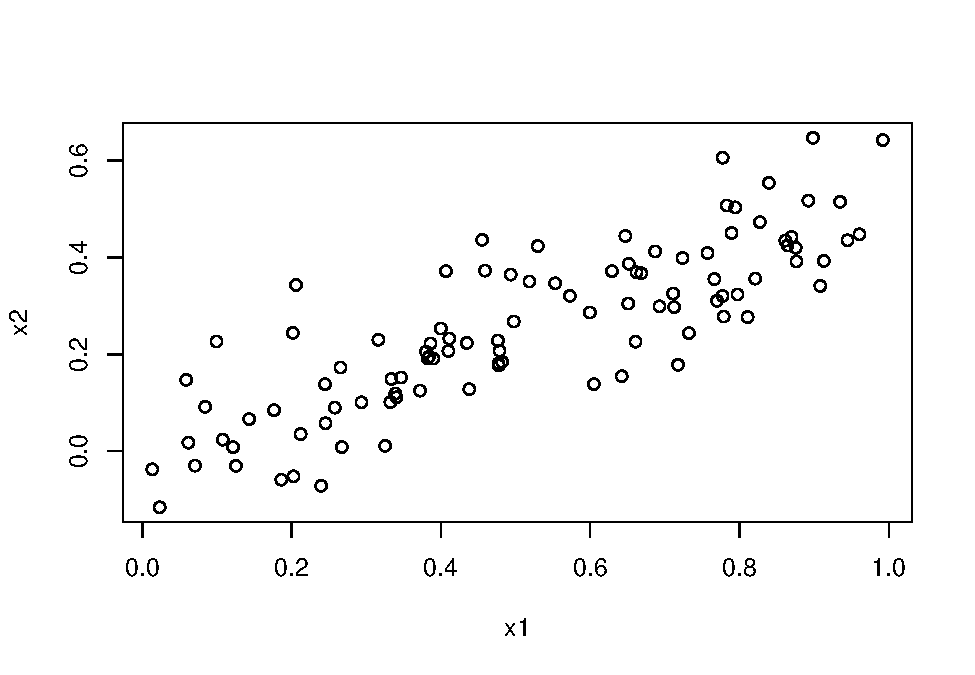
\includegraphics{hw1_fl21_files/figure-latex/unnamed-chunk-17-1.pdf} *
Base on the correlation coefficients, there is an association between
the per capita crime rate \emph{crim} and the other predictors.

\begin{enumerate}
\def\labelenumi{(\alph{enumi})}
\setcounter{enumi}{3}
\tightlist
\item
  Do any of the suburbs of Boston appear to have particularly high crime
  rates? Tax rates? Pupil-teacher ratios? Comment on the range of each
  predictor.
\end{enumerate}

\begin{Shaded}
\begin{Highlighting}[]
\FunctionTok{summary}\NormalTok{(Boston}\SpecialCharTok{$}\NormalTok{crim)}
\end{Highlighting}
\end{Shaded}

\begin{verbatim}
##     Min.  1st Qu.   Median     Mean  3rd Qu.     Max. 
##  0.00632  0.08204  0.25651  3.61352  3.67708 88.97620
\end{verbatim}

\begin{Shaded}
\begin{Highlighting}[]
\NormalTok{selection }\OtherTok{=} \FunctionTok{subset}\NormalTok{(Boston, crim}\SpecialCharTok{\textgreater{}}\DecValTok{10}\NormalTok{)}
\FunctionTok{nrow}\NormalTok{(selection)}\SpecialCharTok{/}\FunctionTok{nrow}\NormalTok{(Boston)}
\end{Highlighting}
\end{Shaded}

\begin{verbatim}
## [1] 0.1067194
\end{verbatim}

\begin{itemize}
\tightlist
\item
  \(11\%\) of the neighborhood's have crime rates that is above \(10%
  \)
\end{itemize}

\begin{Shaded}
\begin{Highlighting}[]
\FunctionTok{summary}\NormalTok{(Boston}\SpecialCharTok{$}\NormalTok{tax)}
\end{Highlighting}
\end{Shaded}

\begin{verbatim}
##    Min. 1st Qu.  Median    Mean 3rd Qu.    Max. 
##   187.0   279.0   330.0   408.2   666.0   711.0
\end{verbatim}

\begin{Shaded}
\begin{Highlighting}[]
\NormalTok{selection }\OtherTok{=} \FunctionTok{subset}\NormalTok{(Boston, tax }\SpecialCharTok{\textless{}} \DecValTok{400}\NormalTok{)}
\FunctionTok{nrow}\NormalTok{(selection)}\SpecialCharTok{/}\FunctionTok{nrow}\NormalTok{(Boston)}
\end{Highlighting}
\end{Shaded}

\begin{verbatim}
## [1] 0.6047431
\end{verbatim}

\begin{itemize}
\tightlist
\item
  \(60.4\%\) of the neighborhood pay under \$400.
\end{itemize}

\begin{Shaded}
\begin{Highlighting}[]
\FunctionTok{summary}\NormalTok{(Boston}\SpecialCharTok{$}\NormalTok{ptratio)}
\end{Highlighting}
\end{Shaded}

\begin{verbatim}
##    Min. 1st Qu.  Median    Mean 3rd Qu.    Max. 
##   12.60   17.40   19.05   18.46   20.20   22.00
\end{verbatim}

\begin{Shaded}
\begin{Highlighting}[]
\NormalTok{selection }\OtherTok{=} \FunctionTok{subset}\NormalTok{(Boston, ptratio }\SpecialCharTok{\textgreater{}} \DecValTok{20}\NormalTok{)}
\FunctionTok{nrow}\NormalTok{(selection) }\SpecialCharTok{/} \FunctionTok{nrow}\NormalTok{(Boston)}
\end{Highlighting}
\end{Shaded}

\begin{verbatim}
## [1] 0.3972332
\end{verbatim}

\begin{enumerate}
\def\labelenumi{(\alph{enumi})}
\setcounter{enumi}{4}
\tightlist
\item
  How many of the suburbs in this data set bound the Charles river?
\end{enumerate}

\begin{Shaded}
\begin{Highlighting}[]
\FunctionTok{nrow}\NormalTok{(}\FunctionTok{subset}\NormalTok{(Boston, chas }\SpecialCharTok{==} \DecValTok{1}\NormalTok{))}
\end{Highlighting}
\end{Shaded}

\begin{verbatim}
## [1] 35
\end{verbatim}

\begin{enumerate}
\def\labelenumi{(\alph{enumi})}
\setcounter{enumi}{5}
\tightlist
\item
  What is the median pupil-teacher ratio among the towns in this data
  set?
\end{enumerate}

\begin{Shaded}
\begin{Highlighting}[]
\FunctionTok{summary}\NormalTok{(Boston}\SpecialCharTok{$}\NormalTok{ptratio)}
\end{Highlighting}
\end{Shaded}

\begin{verbatim}
##    Min. 1st Qu.  Median    Mean 3rd Qu.    Max. 
##   12.60   17.40   19.05   18.46   20.20   22.00
\end{verbatim}

\begin{itemize}
\tightlist
\item
  The median pupil-teacher ratio among the towns is 19.
\end{itemize}

\begin{enumerate}
\def\labelenumi{(\alph{enumi})}
\setcounter{enumi}{7}
\tightlist
\item
  In this data set, how many of the suburbs average more than seven
  rooms per dwelling? More than eight rooms per dwelling? Comment on the
  suburbs that average more than eight rooms per dwelling.
\end{enumerate}

\begin{Shaded}
\begin{Highlighting}[]
\NormalTok{over7rooms }\OtherTok{=} \FunctionTok{subset}\NormalTok{(Boston, rm }\SpecialCharTok{\textgreater{}} \DecValTok{7}\NormalTok{)}
\FunctionTok{nrow}\NormalTok{(over7rooms)}
\end{Highlighting}
\end{Shaded}

\begin{verbatim}
## [1] 64
\end{verbatim}

\begin{itemize}
\tightlist
\item
  There are 64 suburbs that have more than 7 rooms
\end{itemize}

\begin{Shaded}
\begin{Highlighting}[]
\NormalTok{over8rooms }\OtherTok{=} \FunctionTok{subset}\NormalTok{(Boston, rm }\SpecialCharTok{\textgreater{}} \DecValTok{8}\NormalTok{)}
\FunctionTok{nrow}\NormalTok{(over8rooms)}
\end{Highlighting}
\end{Shaded}

\begin{verbatim}
## [1] 13
\end{verbatim}

\begin{Shaded}
\begin{Highlighting}[]
\FunctionTok{summary}\NormalTok{(over8rooms)}
\end{Highlighting}
\end{Shaded}

\begin{verbatim}
##       crim               zn            indus             chas       
##  Min.   :0.02009   Min.   : 0.00   Min.   : 2.680   Min.   :0.0000  
##  1st Qu.:0.33147   1st Qu.: 0.00   1st Qu.: 3.970   1st Qu.:0.0000  
##  Median :0.52014   Median : 0.00   Median : 6.200   Median :0.0000  
##  Mean   :0.71879   Mean   :13.62   Mean   : 7.078   Mean   :0.1538  
##  3rd Qu.:0.57834   3rd Qu.:20.00   3rd Qu.: 6.200   3rd Qu.:0.0000  
##  Max.   :3.47428   Max.   :95.00   Max.   :19.580   Max.   :1.0000  
##       nox               rm             age             dis       
##  Min.   :0.4161   Min.   :8.034   Min.   : 8.40   Min.   :1.801  
##  1st Qu.:0.5040   1st Qu.:8.247   1st Qu.:70.40   1st Qu.:2.288  
##  Median :0.5070   Median :8.297   Median :78.30   Median :2.894  
##  Mean   :0.5392   Mean   :8.349   Mean   :71.54   Mean   :3.430  
##  3rd Qu.:0.6050   3rd Qu.:8.398   3rd Qu.:86.50   3rd Qu.:3.652  
##  Max.   :0.7180   Max.   :8.780   Max.   :93.90   Max.   :8.907  
##       rad              tax           ptratio          black      
##  Min.   : 2.000   Min.   :224.0   Min.   :13.00   Min.   :354.6  
##  1st Qu.: 5.000   1st Qu.:264.0   1st Qu.:14.70   1st Qu.:384.5  
##  Median : 7.000   Median :307.0   Median :17.40   Median :386.9  
##  Mean   : 7.462   Mean   :325.1   Mean   :16.36   Mean   :385.2  
##  3rd Qu.: 8.000   3rd Qu.:307.0   3rd Qu.:17.40   3rd Qu.:389.7  
##  Max.   :24.000   Max.   :666.0   Max.   :20.20   Max.   :396.9  
##      lstat           medv     
##  Min.   :2.47   Min.   :21.9  
##  1st Qu.:3.32   1st Qu.:41.7  
##  Median :4.14   Median :48.3  
##  Mean   :4.31   Mean   :44.2  
##  3rd Qu.:5.12   3rd Qu.:50.0  
##  Max.   :7.44   Max.   :50.0
\end{verbatim}

\begin{itemize}
\tightlist
\item
  There are 13 suburbs that have more than 13 rooms
\end{itemize}

\end{document}
